%%%%%%%%%%%%%%%%%%%%%%%%%%%%%%%%%%%%%%%%%%%%%%%%%%%%%%%
%% Engineer & Master Thesis, LaTeX Template          %%
%% Copyleft by Piotr Woźniak & Artur M. Brodzki      %%
%% Faculty of Electronics and Information Technology %%
%% Warsaw University of Technology, Warsaw, 2019     %%
%%%%%%%%%%%%%%%%%%%%%%%%%%%%%%%%%%%%%%%%%%%%%%%%%%%%%%%

\documentclass[
    left=2.5cm,         % Sadly, generic margin parameter
    right=2.5cm,        % doesnt't work, as it is
    top=2.5cm,          % superseded by more specific
    bottom=3cm,         % left...bottom parameters.
    bindingoffset=6mm,  % Optional binding offset.
    nohyphenation=false % You may turn off hyphenation, if don't like.
]{eiti/eiti-thesis}

\langpol % Dla języka angielskiego mamy \langeng
\graphicspath{{img/}}             % Katalog z obrazkami.
\addbibresource{bibliografia.bib} % Plik .bib z bibliografią

\begin{document}

%--------------------------------------
% Strona tytułowa
%--------------------------------------
\MasterThesis % dla pracy inżynierskiej mamy \EngineerThesis
\instytut{XXXXXX}
\kierunek{XXXXXX}
\specjalnosc{XXXXXX}
\title{
    Niepotrzebnie długi i skomplikowany tytuł pracy \\
    trudny do przeczytania, zrozumienia i wymówienia
}
\engtitle{ % Tytuł po angielsku do angielskiego streszczenia
    Unnecessarily long and complicated thesis' title \\
    difficult to read, understand and pronounce
}
\author{\{Imię i Nazwisko\}}
\album{XXXXXX}
\promotor{XXXXXX}
\date{\the\year}
\maketitle

%--------------------------------------
% Streszczenie po polsku
%--------------------------------------
\cleardoublepage % Zaczynamy od nieparzystej strony
\streszczenie \lipsum[1-3]
\slowakluczowe XXX, XXX, XXX

%--------------------------------------
% Streszczenie po angielsku
%--------------------------------------
\newpage
\abstract \kant[1-3]
\keywords XXX, XXX, XXX

%--------------------------------------
% Oświadczenie o autorstwie
%--------------------------------------
\newpage
\makeauthorship

%--------------------------------------
% Spis treści
%--------------------------------------
\cleardoublepage % Zaczynamy od nieparzystej strony
\pagestyle{plain}
\tableofcontents

%--------------------------------------
% Rozdziały
%--------------------------------------
\cleardoublepage % Zaczynamy od nieparzystej strony
\pagestyle{headings}

% Wygodnie jest trzymać każdy rozdział w osobnym pliku.
% Umożliwia to również łatwą migrację do nowej wersji szablonu:
% wystarczy podmienić swoje pliki main.tex i eiti-thesis.cls
% na nowe wersje, a cały tekst pracy pozostaje nienaruszony.
\newpage % Rozdziały zaczynamy od nowej strony.
\section{Zbiory danych} \label{dane_wejsciowe}

%todo:
% \colorbox{yellow}{todo:}\\

% //todo: opisać te kategrię ironii z uwzględniem kategorii z wczesniejszego rodziału
% // to z biegunowości i bez to są dwa typy ironii verbalnej -> tylko jedno z nich jest trudniejsze z punktu widzenia zagadanienai kalsyfikacji

W ramach pracy zostały wykorzystane dwa zbiory danych. Pierwszy zbiór danych (w pracy oznaczony jako zbiór A) został udostępniony w ramach inicjatywy SemEval. Inicjatywa ta ma na celu rozwój szeroko pojętej analizy i przetwarzania języka naturalnego. Zbiór ten składa się 4618 próbek oznaczonych tagiem o klasyfikującym rekord jako ironiczny lub nie. Dane pochodzą z Twittera i reprezentują trzy różne typy ironii:
\begin{itemize}
    \item Słowną werbalną stworzoną poprzez wykorzystaniu przeciwnej biegunowości słów (polarity contrast):
          \begin{itemize}
              \item Przykład: I love waking up with migraines \#not :'(
          \end{itemize}

    \item Słowną werbalną stworzoną bez wykorzystania przeciwnej biegunowości:
          \begin{itemize}
              \item Przykład: Human brains disappear every day. Some of them have never even appeared. \#brain \#humanbrain \#Sarcasm
          \end{itemize}

    \item Ironia sytuacyjna:
          \begin{itemize}
              \item Przykład: Most of us didn't focus in the \#ADHD lecture. \#irony
          \end{itemize}
\end{itemize}



Drugi zbiór (w pracy oznaczony jako zbiór B) także pochodzi z Twittera i został zebrany w ramach publikacji zajmującej się analizą różnic między sarkazmem, a ironią  \cite{Ling2016}  , badacze zebrane dane podzielili na 4 zbiory, każdy o zawierający 30 tysięcy próbek,  reprezentujące poniższe kategorie:
\begin{itemize}
    \item Ironiczny
    \item Sarkastyczny
    \item Zmieszany zbiór ironiczny i sarkastyczny
    \item Niezawierający ani ironii, ani sarkazmu

\end{itemize}

Każdy rekord w ramach zbioru danych posiadał następujące informacje:
\begin{itemize}
    \item datą opublikowania
    \item nazwę użytkownika
    \item unikalny ID Tweetu
\end{itemize}


%todo
% \colorbox{yellow}{todo:}\\

% //todo: lista paramterów

Ze względu na to, że wiadomość zawarta w ramach Tweetu nie była podana wprost, tylko sprecyzowany był jej unikalny ID, konieczne było dokonanie dodatkowego mapowania między rekordami, a postami wykorzystując udostępnione przez Tweeter API. Podczas procesu mapowania nie udało się uzyskać wszystkich treści postów, część z nich była nie osiągalna ze względu na różne czynniki losowe takie jak usuniecie konta użytkownika, zablokowanie Tweetu ze względu na naruszenie regulaminu portalu oraz usunięcie Tweetu przez użytkownika. Dlatego uzyskany zbiór postów był mniejszy od 30 tysięcy.  
Na potrzeby pracy zostały wykorzystane 2 zbiory z wcześniej wymienionych:
\begin{itemize}
    \item Zmieszany zbiór ironiczny i sarkastyczny -> zbiór posiadał 22402 próbek
    \item Niezawierający ani ironii, ani sarkazmu -> zbiór posiadł 19018 próbek
\end{itemize}



\newpage % Rozdziały zaczynamy od nowej strony.
\section{Embeddingi} \label{embeddings}

\subsection{Co to jest embedding słów}
% zrodło https://towardsdatascience.com/neural-network-embeddings-explained-4d028e6f0526
% zrodlo 2 https://www.tensorflow.org/tutorials/text/word_embeddings
% -----  https://developers.google.com/machine-learning/crash-course/embeddings/video-lecture

% ---- https://en.wikipedia.org/wiki/Word_embedding

% https://pathmind.com/wiki/glossary#cosine

% https://machinelearningmastery.com/what-are-word-embeddings/


Embedding słów jest to zbiorcza nazwa na techniki i narzędzia wykorzystane w ramach przetwarzania języka naturalnego pozwalające na dokonanie mapowania słów, ze zbioru znanych pojęć, na wektor liczb rzeczywistych. Z matematycznego punktu widzenia sprowadza się to do transformacji z dyskretnej przestrzeni o wielu wymiarach do ciągłej przestrzeni ze znacznie mniejszą liczbą wymiarów. 
% zrodlo ----> https://en.wikipedia.org/wiki/Word_embedding

%Word embedding is the collective name for a set of language modeling and feature learning techniques in natural language processing (NLP) where words or phrases from the vocabulary are mapped to vectors of real numbers. Conceptually it involves a mathematical embedding from a space with many dimensions per word to a continuous vector space with a much lower dimension.


Takie podejście powoduje, że możliwe jest badanie podobieństwa słów wykorzystując cosinusowe podobieństwo. Jeśli dwa słowa mają podobne znaczenia lub wykorzystywane są w podobnym kontekście  wartość podobieństwa będzie bliższa jednemu. Jeśli słowa rzadko ze sobą występują wartość podobieństwa będzie bliższa zera. 

%todo: można dodać wzór na liczenie...



%zrodlo -> https://www.tensorflow.org/tutorials/text/word_embeddings

%Word embeddings give us a way to use an efficient, dense representation in which similar words have a similar encodin



\subsection{Wykorzystane embeddingi}
W ramach pracy są wykorzystywane trzy rodzaje embeddingów, każdy z nich różni się długością wektora i sposobem jego uzyskania. Wykorzystane w pracy embeddingi to:
\begin{itemize}
    % \item Word2vec
    \item Glove
    \item FastText
    \item ELMo
\end{itemize}



\subsubsection{Word2vec}
Metoda ta nie została wykorzystana w pracy, jednak jest ona kluczowy do zrzumienia podstaw działania i tworzenia ebeddingów dlatego zostanie omówiony w tej sekcji. Występuje w dwóch odmianach: 

\begin{itemize}
    \item CBOW
    \item skip grams 
\end{itemize}



Tworzenie embeddingu w oparciu o model typu CBOW polega na trenowaniu prostej sieci neuronowej. Sieć ta składa się z warstwy wejściowej, jednej warstwy ukrytej (w gęstej) oraz warstwy wyjściowej. Trening modelu polega na podawaniu na wejście słów mieszczących się w ramach pewnego założonego okna, przewidując słowo będące w środku tego okna. Jako okno rozumie się tutaj stałą liczbę słów przed i po aktualnie przewidywanym słowie. Słowa, by mogły być przewidywane przez model, są wcześniej konwertowane do przestrzeni wektorowej poprzez wykorzystanie one-hot encodingu. Proces uczenia polega na systematycznym przesuwaniu okna o jedno słowo i trenowanie wag w warstwie ukrytej. Po zakończonym procesie uczenia należy usunąć ostatnią warstwę wyjściową, a wagi z warstwy ukrytej pozwalają na uzyskanie embeddingu słów.  

Odmiana ‘skip grams’ jest analogiczna do metody CBOW, tylko zamiast przewidywania jednego słowa w kontekście jego otoczenia, przewidywane jest otoczenie w kontekście słowa. 


\subsubsection{Glove}
% https://nlp.stanford.edu/pubs/glove.pdf

Metoda opiera na wykorzystaniu globalnych statystyk współwystępowania słów, zamiast wykorzystywania tylko informacji o lokalnym kontekście, jak jest to czynione w ramach metody word2vec. Współwystępowanie słów jest zliczane w ramach stałego okna, w ramach które wchodzi skąd 10 słów z lewej i z prawej strony. 

Trenowanie modelu polega na wyznaczeniu takich embeddingów słów by ich iloczyn skalarny był równy logarytmowi prawdopodobieństwa współwystępowania tych słów w korpusie. Jest to opisane poniższymi wzorami: 

%todo
//wstwaić wzór i opisać jego elementy 

\begin{figure}[!h]
    \label{fig:wzor}
    \centering 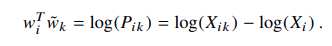
\includegraphics[width=0.5\linewidth]{Selection_016.png}
    \caption{Wzór: //todo: do przeniesiania dolatexa}
\end{figure}

\subsubsection{FastText}

Embedding FastText został stworzony w ramach badań prowadzonych przez firmę Facebook. Jest on wariacją metody word2vec, która rozważa zdanie na jeszcze niższym poziomie. Metoda ta rozbija słowa na jeszcze mniejsze fragmenty, tzw. n-gramy. Dla przykładu, angielskie słowo ‘where’ (dla okna o wielkości n=3) jest rozbijane na następujące części: <wh, whe, her, ere, re>. Badacze dodali także specjalne symbole ‘<’ oraz ‘>’ pozwalające poprawnie identyfikować przedrostki i przyrostki. Także by zachować informację o pełnej formie słowa, słowo to jest także dodane do zbioru n-gramów. 

Tak uzyskana interpretacja słowa jest konwertowana do postaci numerycznego wektora. Polega to na dodawaniu wektorów kolejnych elementów zbioru n-gramów do jednego długiego wektora. Tak uzyskane wektory poszczególnych słów są podawane analogicznie jak w przypadku tradycyjnego word2vec na wejścia płaskiej sieci pozwalając finalnie wyznaczyć embeddingi słów. 

% https://arxiv.org/pdf/1607.04606.pdf
% Enriching Word Vectors with Subword Information

\subsubsection{ELMo}

Ta metoda tworzenia embeddingów nie korzysta już z bezpośrednio z podwalin stworzonych przez metodę word2vec. Zamiast tego do wychwytywania kontekstu słowa, niezbędnego do stworzenia poprawnych embeddingów, wykorzystuje warstwy LSTM. Warstwa ta dzięki swojej budowie pozwala na efektywne zapamiętywanie istotnych informacji, z punktu widzenia zagadnienia klasyfikacji, pojawiających się wcześniej w ramach sekwencji danych wejściowych. 
%todo
//wiecej szczeŋółów rozdział o wartwaych  ->odnośnik

 

Przetwarzanie zdania wejściowego odbywa się zgodnie z następującymi krokami: 

\begin{itemize}
    \item Zdanie jest dzielone na słowa 
    \item Każde słowo, przy wykorzystaniu sieci pomocniczej typu CNN(opierającej się o warswy konwolucyjne), ma przypisywany embedding. Embedding ten jest określany poprzez agregację wektorowej reprezentacji pojedynczych znaków występujących w ramach słowa. Tak uzyskany embedding jest pierwszym elementem finalnego embeddingu (oznaczony jako $E_1$)
    \item Uzyskany wektor jest podawany na wejście pierwszej warstwy Bi-LSTM. Warstwa ta pozwala na analizę zdania zarówno od początku do końca, jak i od końca do początku. 
    \item  Stany ukryte z pierwszej warstwy dla każdego słowa są agregowane w jeden wektor i stanowią drugi element finalnego embeddingu (oznaczony jako $E_2$) 
    \item Następnie dane o stanie ukrytym pierwszej warstwy są przekazywane na drugą warstwę Bi-LSTM 
    \item Stany ukryte z drugiej warstwy dla każdego słowa są agregowane w jeden wektor i stanowią drugi element finalnego embeddingu (oznaczony jako $E_3$) 
    \item W ostaniem kroku następuje połącznie uzyskanych fragmentów embeddingów, oznaczonych jako $E_1,E_2, E_3$ w jeden o standardowym wymiarze 1024 
\end{itemize}

 

% //todo: dodać rysunek arch -> bo jest duża fajnych 


%todo: opisać czym są postagi
\subsection{Uwzględnienie POS tagów w ramach embeddingu}


POS tag (Part-of-speach tag) zawiera informacje na temat cech morfosyntatycznych słowa. Najbardziej podstawową kategorią są powszechnie znane części mowy, takie jak czasownik, rzeczownik, przymiotnik. Jednak nie jest to jedyna informacja zawarta w ramach takiego tagu, przechowuje on bowiem także informację o czasie w jakim jest użyty czasownik, w której liczbie jest wykorzystany rzeczownik i wiele innych.  

%todo:
//todo: można by dorzucić pełną listę, ale to może być problematyczne 
% tu jest lista: https://medium.com/@gianpaul.r/tokenization-and-parts-of-speech-pos-tagging-in-pythons-nltk-library-2d30f70af13b
 
% https://pythonprogramming.net/natural-language-toolkit-nltk-part-speech-tagging/

Aby umieścić informacje na temat części mowy tak by była ona możliwa do interpretacji w ramach embeddingu konieczne jest konwertowanie jej do postaci wektorowej. Ze względu na brak dużego podobieństwa między poszczególnymi częściami mowy zdecydowano się na zakodowanie tej informacji w formie one-hot encoding. Tak utworzony wektor był doklejany do istniejącego już embeddingu uzyskanego innymi metodami tworząc wektor dłuższy o 46 elementów. 

%todo:
//todo: dodać rysunek to obrazujący
\newpage % Rozdziały zaczynamy od nowej strony.
\section{Preprocessing}

Aby zapewnić jak najlepszą jakość klasyfikacji konieczne jest obrobienie danych do postaci pozbawionej zbędnych szumów. Na potrzeby tej pracy zostały podjęte następujące kroki obróbki danych:

%MOżna napisać czyimi pracami się sugerowałem pisząc preprocessing

\begin{enumerate}
    \item Zastąpienie linków tagiem “<url>”.
    \item Usunięcie znaków końca linii.
    \item Zastąpienie wystąpień nazw użytkowników tagiem  “<username>”.
    \item Zamiana emotikon z formatu “:XX\_YY:” na format “<emote> XX YY” .
    \item Rozbicie hasztagów na mniejsze słowa, oznaczenie go tagiem “<hashtag>”.
    \item Zastąpienie oznaczeń odnoszących się do czasu tagiem “<time>”.
    \item Zastąpienie liczb tagiem “<number>”.
    \item Usunięcie znaków  '' | ''  oraz wielokropków.
    \item Konwersja do małych liter.
    \item Rozwinięcie form skróconych do ich pełnych form.
\end{enumerate}

\begin{table}[!h] \label{tab:tabela2} \centering
    \caption{Tabela przedstawiająca efekt preprocessingu.}
    \begin{tabular} {| c | c | c |} \hline
        Numer operacji preprocessingu & Przed konwersją                                          & Po konwersji                   \\ \hline\hline
        1                             & www.google.pl                                            & <url>                          \\ \hline
        2                             & \textbackslash n \quad \textbackslash r \textbackslash n &                                \\ \hline
        3                             & @mike                                                    & <username>                     \\ \hline
        4                             & :face\_screaming\_in\_fear:                              & <emote> face screaming in fear \\ \hline
        5                             & \#trueFriend                                             & <hashtag> true Friend          \\ \hline
        6                             & 14:58                                                    & <time>                         \\ \hline
        7                             & 1234                                                     & <number>                       \\ \hline
        8                             & | ...                                                    & .                              \\ \hline
        9                             & Kazimierz Wielki                                         & kazimierz wielki               \\ \hline
        10                            & I'll \quad | \quad He's                                  & I will \quad | \quad He has    \\ \hline
    \end{tabular}
\end{table}

%todo:
% być może warto opisać w jaki sposób robię te operacje usuwania ?? -> że regexxy
% być może warto opisać o tych formach skróconych, że to model dodakowy wychwytuje
% można teżnapisać czemu nie wykorzystuję stremingu i lematyzacji
%



\newpage % Rozdziały zaczynamy od nowej strony.
\section{Struktura sieci}

\subsection{Warstwa gęsta}

%http://zsi.tech.us.edu.pl/~nowak/si/SI_w4.pdf 

%https://www.fuw.edu.pl/~jarekz/SIECI/wyklad3.pdf 

Jest to najbardziej podstawowy typ warstwy, w której każdy neuron uzyskuje informacje ze wszystkich wejść. Następnie agreguje te dane, przy uwzględnieniu wag odpowiadającym wejściom i przy wykorzystaniu swojej funkcji aktywacji wylicza wartość wyjściową neuronu\cite{dense_1}. 

Często jedna warstwa gęsto połączona nie wystarcza by poprawnie rozwiązywać dane zadanie klasyfikacji, dlatego wykorzystuje się kilka takich warstw ze sobą połączonych tak, że wyjścia jednej warstwy są jednocześnie wejściami kolejnej warstwy. Należy jednak pamiętać, że funkcja aktywacji musi być wtedy funkcją nieliniową\cite{dense_2}. Obecnie najczęściej wykorzystywaną funkcją aktywacji jest funkcja ReLU opisana poniższym wzorem\cite{acct_func}: 

%https://en.wikipedia.org/wiki/Activation_function
$$f(x) = max(0,x) = \left\{\begin{matrix}
         & 0,\ dla\ x \leq 0 \\
         & x,\ dla\ x > 0
    \end{matrix}\right.
$$

\subsection{Warstwa konwolucyjna}

% https://towardsdatascience.com/text-classification-rnns-or-cnn-s-98c86a0dd361
% https://towardsdatascience.com/a-comprehensive-guide-to-convolutional-neural-networks-the-eli5-way-3bd2b1164a53

% http://www.wildml.com/2015/11/understanding-convolutional-neural-networks-for-nlp/

Sieci używające warstw konwolucyjnych (takie sieci oznaczane są często jako CNN) z reguły wykorzystywane są w ramach analizy obrazu. Działają one w oparciu o różne filtry przemieszczające się systematycznie po macierzy obrazu. Dany obraz może być jednocześnie analizowany przez wiele filtrów przemieszczających się z różnym skokiem. Pozwala to na naukę rozpoznawania różnych cech obrazu umożliwiających zagadnienia klasyfikacji. Kolejne warstwy konwolucyjne można ze sobą łączyć pozwalając na rozpoznawanie coraz bardziej zaawansowanych cech obrazu\cite{cnn_1} \cite{cnn_2}.

W przypadku analizy tekstu macierzą wejściową dla warstwy konwolucyjnej jest macierz o wymiarze AxB, gdzie A to liczba słów w zdaniu, a B to rozmiar reprezentacji wektorowej słowa. Natomiast, ze względu na strukturę danych, sama ekstrakcja cech dokonywana przez filtr może przebiegać tylko w ramach wymiaru A, gdyż dane wzdłuż wymiaru B reprezentują unikalne cechy danego słowa i nie powinny być agregowane\cite{cnn_3}.


\subsection{Pooling}

%https://www.quora.com/What-is-pooling-in-a-convolutional-neural-network 

%https://www.quora.com/What-is-max-pooling-in-convolutional-neural-networks 

Zadaniem warstwy poolingu jest zmniejszenie wymiarowości macierzy uzyskanej z poprzedniej warstwy (bardzo często występuję tuż po warstwie konwolucyjnej). Można ten proces porównać do przeprowadzania operacji zmniejszania rozdzielczości obrazu. Operacja ta polega na systematycznym przesuwaniu stałego okna po macierzy wejściowej i dokonywania pewnej formy agregacji danych (wybór elementu o najwyższej wartości, wyliczenie średniej z wartości elementów) na elementach macierzy zawierających się w bieżącym oknie. Dzięki takiemu zabiegowi kolejne warstwy sieci mogą skupiać się na analizie i wykrywaniu bardziej skomplikowanych wzorców w oparciu o cechy uwypuklone przez warstwę poolingu. \cite{pooling_1} \cite{pooling_2}

 

Najbardziej popularną formą poolingu jest max pooling, który polega na wybieraniu elementu o najwyższej wartości spośród elementów w oknie. Na rysunku \ref{fig:max_pooling} przedstawiono przykład takiej operacji przy zastosowaniu okna o rozmiarze 2x2 i przesunięciu wynoszącym 2. 

\begin{figure}[!h]
    \centering 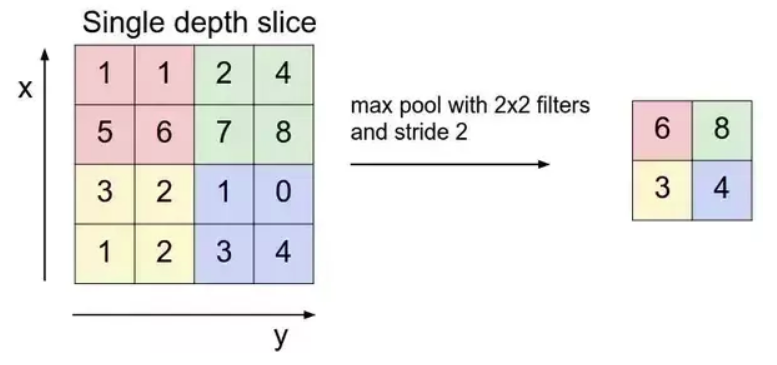
\includegraphics[width=0.75\linewidth]{max_pooling.png}
    \caption{Wynik operacji max poolingu\cite{pooling_2}}
    \label{fig:max_pooling}
\end{figure}


\subsection{RNN}

% http://colah.github.io/posts/2015-08-Understanding-LSTMs/ 

% https://towardsdatascience.com/illustrated-guide-to-recurrent-neural-networks-79e5eb8049c9 


Neuronowa sieć rekurencyjna (RNN) powstała z myślą o przewidywaniu kolejnych elementów sekwencji. Jako wejście przyjmuje kolejne elementy sekwencji, ale w przeciwieństwie do sieci typu feedforward posiada także swój wewnętrzny  stan, w ramach którego zawarta jest informacja o poprzednich wejściach. Sieć tego typu charakteryzuje się jednak bardzo istotną wadą, mianowicie boryka się ona z problem zanikającego gradientu. Jest on spowodowany naturą propagacji wstecznej i wiąże się z coraz mniejszym wpływem początkowych elementów sekwencji na wyjście modelu. Aby temu zaradzić zostały wprowadzone nowe architektury warstw, jedną z nich jest warstwa typu LSTM. \cite{RNN_1} \cite{RNN_2}




\subsection{\label{lstm_subsection}LSTM}



% https://towardsdatascience.com/illustrated-guide-to-lstms-and-gru-s-a-step-by-step-explanation-44e9eb85bf21

Warstwa typu LSTM składa się nuronów zawierających w sobie wiele pośrednich operacji. Poniżej zostaną omówione najważniejsze z nich \cite{LSTM_1}.

\begin{figure}[!h]
    \label{fig:lstm_diagram}
    \centering 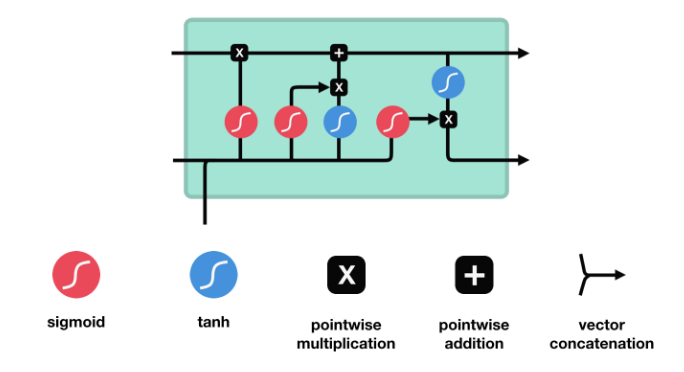
\includegraphics[width=0.6\linewidth]{lstm_diagram.png}
    \caption{Przepływ danych w pojedynczym neuronie LSTM \cite{LSTM_1}}
\end{figure}




\subsubsection{Funkcje aktywacji}

Neuron LSTM wykorzystuje dwie funkcje aktywacji:

\begin{itemize}
    \item Tahn (funkcja aktywacji typu tangens hiperboliczny) - pozwala ona na normalizowanie wektora tak by wartości zawierały się w ramach przedziału [-1,1]
    \item Sigmoid (funkcja aktywacji sigmoidalna) - przekształca wartości wektora do wartości z przedziału [0,1]. Istotna z punktu widzenia określania, które elementy wektora powinny zostać zapamiętane (wartość bliżej 1), a które zapomniane (wartość bliżej 0)
\end{itemize}


\subsubsection{Elementy neuronu}

W skład neuronu LSTM wchodzą następujące elementy:
\begin{itemize}
    \item Forget gate
    \item Input gate
    \item Cell state
    \item Output gate
\end{itemize}

\begin{figure}[!h]
    \label{fig:lstm_gates}
    \centering 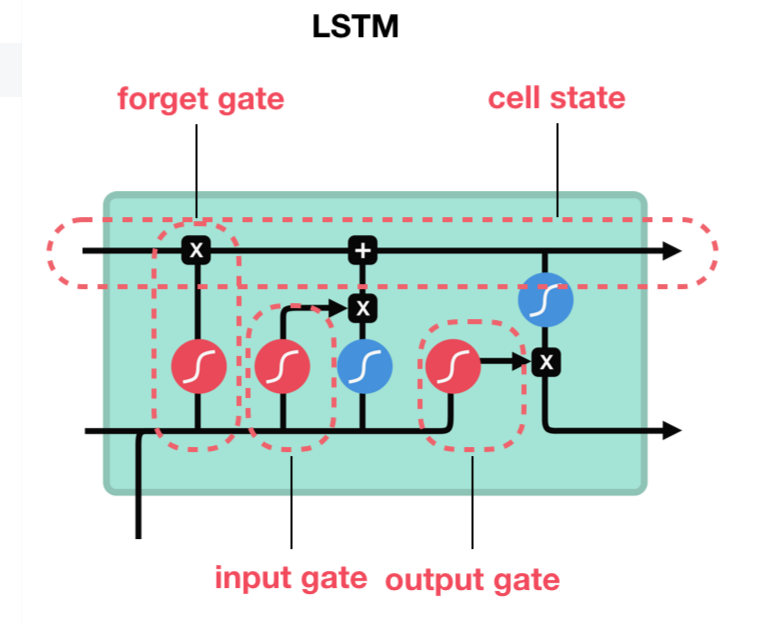
\includegraphics[width=0.5\linewidth]{lstm_gates.png}
    \caption{Elementy wewnątrz neuronu LSTM \cite{LSTM_1}}
\end{figure}

\paragraph{Forget gate}  \hfill
%  \break

Zadaniem tej bramy jest decydowanie jaka informacja powinna zostać zachowana przez neuron, a jaka usunięta. Informacje z poprzedniego stanu ukrytego ($h_{t-1}$) i informacje z bieżącego wejścia($x_t$) są przekazywane do sigmoidalnej funkcji aktywacji. Powstała macierz jest oznaczona jako $f_t$. Dla każdej pozycji w macierzy zwracane są wartości z zakresu [0,1]. Im bliżej wartości zero, tym wpływ danej pozycji zanika, im bliżej wartości jeden tym wpływ danej pozycji rośnie.


\paragraph{Input gate}  \hfill

Służy do aktualizacji wewnętrznego stanu neuronu (‘cell state’). Informacje z poprzedniego stanu ukrytego ($h_{t-1}$) i informacje z bieżącego wejścia($x_t$) są przekazywane do sigmoidalnej funkcji aktywacji. Tak jak w przypadku 'forget gate’ uzyskiwana jest macierz o wartościach z zakresu [0,1], która tym razem określa jak bardzo informacja, powstała z połącznia $h_{t-1}$ oraz $x_t$, jest ważna z punktu widzenia zadania klasyfikacji. Wyjście z tej operacji oznaczone jest jako $i_t$.

W ramach tej bramy dokonuje się normalizacja informacji zawartych w ramach połączenia $h_{t-1}$ oraz $x_t$, poprzez wykorzystanie tangensa hiperbolicznego. Wyjście z tej operacji oznaczone jest jako $c_t$.

Kolejnym krokiem jest agregacja informacji z $i_t$ oraz $c_t$ poprzez wykonanie operacji mnożenia macierzy.

\paragraph{Cell state}  \hfill

Ten element neuronu odpowiada za jego stan wewnętrzny i jest przekazywany między kolejnymi komórkami w warstwie. Stan uzyskany z poprzedniej komórki oznaczony jest jako $c_{t-1}$, a z bieżącej jako $c_t$. W celu uzyskania bieżącego stanu komórki wykorzystywane są informacje zgromadzone w ramach poprzednich bram. W pierwszej kolejności dokonywane jest mnożenie macierzowe $c_{t-1}$ oraz $f_t$, które pozwala na usunięcie elementów macierzy nieistotnych z punktu widzenia sieci. Następnie dokonywana jest operacja dodawania uzyskanej macierzy z macierzą uzyskaną w ramach ‘input gate’. Powoduje to dodanie do stanu neuronu nowych informacji istotnych dla sieci. Stan po tej operacji jest określany zmienną $c_t$.


\paragraph{Output gate}  \hfill

Zadaniem tej bramy jest określenie jak powinien wyglądać stan ukryty przekazywany do kolejnego neuronu. Stan ten zawiera informacje na temat poprzednich wejść istotnych z dla zagadnienia klasyfikacji. W ramach tej bramy dokonywane są trzy operacje. Pierwszą z nich jest podanie zagregowanych informacji z poprzedniego stanu ukrytego ($h_{t-1}$) i informacje z bieżącego wejścia($x_t$) na sigmoidalną funkcję aktywacji. W ramach drugiej operacji wewnętrzy stan neuronu (‘cell state’) jest normalizowany przy wykorzystaniu tangesna hiperbolicznego. Trzecią operacją jest mnożenie macierzowe wyników dwóch poprzednich operacji, w efekcie uzyskiwany jest stan ukryty neuronu, oznaczony jako $h_t$, przekazywany do następnego neuronu.

\subsection{Bi-LSTM}

%https://medium.com/@raghavaggarwal0089/bi-lstm-bc3d68da8bd0 

Warstwa składa się z dwóch tak samo zbudowanych warstw LSTM. Jedna z warstw przetwarza ciąg danych wejściowych od początku do końca, a druga od końca do początku. Pozwala to na naukę zależności między elementami w dwóch kierunkach, co przekłada się na większą liczbę informacji na temat sekwencji, co pozwala na szybsze i dokładniejsze trenowanie modelu\cite{BI_LSTM_1}.






\newpage % Rozdziały zaczynamy od nowej strony.
\section{Eksperymenty}

\colorbox{yellow}{todo: opisać to jakoś sensownie, punkt po punkcie co i dlaczego robię, bo teraz jest tak mega chatycznie, że nie da sie nic wywniskować}\\

//dlaczego takie sieci został ywybran, dlaczeg otakimi paramterami steruję -> na co powinny one wpływać

%W ramach pracy została dokonana analiza wpływu oznaczeń morfosyntaktycznych na jakość klasyfikacji tekstów ironicznych. Na potrzeby języka angielskiego taka analiza sprowadza się głownie do analizy wpływu typu części mowy do jakiego należą poszczególne słowa i taka analiza zostanie podjęta w kolejnych krokach.

% \colorbox{yellow}{highlight}\\

Na potrzeby analizy wykorzystano wiele różnych modeli sieci neuronowych, bazujących głownie na trzech typach warstw:

\begin{itemize}
    \item gęstej;
    \item konwolucyjnej;
    \item LSTM;
\end{itemize}

W ramach różnych architektur testowany był wpływ kilku hiperparametrów na jakość klasyfikacji. Oto lista niektórych z nich:
\begin{itemize}
    \item dla warstwy gęstej:
          \begin{itemize}
              \item  1/2/3 warstwy
              \item Z dropoutem / bez dropoutu
              \item Wielkość wartwy ukrytej 30-200
          \end{itemize}

    \item dla warstwy konwolucyjnej;
          \begin{itemize}
              \item  1/2/3 warstwy
              \item Wielkość okna 3-15
              \item Z dropoutem / bez dropoutu
              \item Wielkość wartwy ukrytej 30-200
          \end{itemize}
    \item dla warstwy LSTM;
          \begin{itemize}
              \item Wykorzystanie warstwy pojedynczej (LSTM) oraz podwójnej (Bi-LSTM)
              \item  1/2/3 warstwy
              \item Z dropoutem / bez dropoutu
              \item Wielkość wartwy ukrytej 30-200
          \end{itemize}
\end{itemize}

% \subsection{POSTAGS}
% %todo:
% //todo: zmergować z dugim rozdiałem o postagach

% Aby możliwe było wykorzystanie przez sieć neuronową informacji na temat typu części mowy danego słowa konieczne są następujące kroki:

% \begin{enumerate}
%     \item Rozpoznanie części mowy w kontekście zdania i przypisanie do niego odpowiedniego tagu,
%     \item Konwersja wykrytego tagu do liczbowej reprezentacji wektorowej,
%     \item Dołączenie utworzonego wektora do przetrenowanego wektora embedingów.
% \end{enumerate}

% \hfill \break % to dodaje pustą linie po czymść dziwnym -lista, tabela
% Do rozpoznania części mowy zostało wykorzystane narzędzie z pakietu NLTK, które pozwala na oznaczenie każdego słowa w zdaniu jednym z 46 tagów, każdy odpowiadający innej części mowy. Następnie wykryty tag został przetworzony do postaci “one-hot encoding” i dodany do istniejącego embedingu słowa, zwiększając tym samy jego rozmiar o długość 46.


\subsection{Wyniki analiza}

\subsubsection{Eksperyment 1}
% Aby w pełni zweryfikować wpływ części mowy (POS tagów) na jakość klasyfikacji zostały wykorzystane trzy różne embeddingi oraz dwa różne zbiory danych wejściowych. Embeddingi różnią się one między innymi długością oraz metodą ich uzyskiwania. A zbiory danych różnią się licznością i stopniem zaszumienia. Każdy ze zbiorów danych został podzielony na trzy zbiory treningowy, walidacyjny oraz testowy w proporcjach 60/20/20 procent.

Aby w pełni zweryfikować wpływ części mowy (POS tagów) na jakość klasyfikacji zostały wykorzystane trzy różne embeddingi oraz dwa różne zbiory danych wejściowych. Wykorzsytane embeddingi to: Glove, FastText oraz ELMo, a ich dokładniejszy opis znajduje się w rozdziale \ref{embeddings}. Natomiast dwa zbiory danych wejściowych (oznaczonych jako A oraz B) są opisane w rozdziale \ref{dane_wejsciowe}. Na potrzeby budowania modeli każdy ze zbiorów danych został podzielony na trzy podzbiory: treningowy, walidacyjny oraz testowy w proporcjach 60/20/20 procent.

% Poniżej przedstawiono tabele z wynikami obliczeń.
Wyniki uzyskane przez modele na danych testowych zbioru A zostały umiszczone w rozdziale \ref{wyniki_eksperymentow} w tabelach \ref{tab:wyniki_glove_A}, \ref{tab:wyniki_fasttext_A}, \ref{tab:wyniki_elmo_A} , a dla zbioru B w tabelach \ref{tab:wyniki_glove_B}, \ref{tab:wyniki_fasttext_B}, \ref{tab:wyniki_elmo_B}.


W oparciu o uzyskane wyniki można stwierdzić, że wraz z dołączeniem informacji o częściach mowy nie obserwuje się widocznej poprawy jakości klasyfikacji, czasem występuje nawet jej pogorszenie. Jednym z powodów takiego zachowania może być fakt, że rodzaj części mowy nie jest kluczowy do rozpoznania ironicznego charakteru tekstu. Możne to być też spowodowane tym, że sieci wychwytują niezbędne dla nich informacje na temat roli konkretnego słowa w zdaniu w oparciu o uzyskiwany kontekst i dodatkowa informacja w ramach embeddingu jest już niepotrzebna.

Ponadto można zaważyć, że wraz ze wzrostem rozmiaru embedingów poprawia się jakość klasyfikacji, co jest zgodne z oczekiwaniami, jako że dłuższy embedding pozwala na zachowanie większej liczby informacji na temat słowa.


Analizując uśrednione pomiary jakości klasyfikacji dla sieci opartych o różne typy warstw, można zauważyć, że najgorzej sprawują się sieci oparte o warstwy gęste. Natomiast sieci wykorzystujące warstwy konwolucyjne oraz LSTM posiadają podobną skuteczność klasyfikacji. Aby wykluczyć wpływ zaszumienia danych oraz przeuczenia sieci wykonano jeszcze dwa eksperymenty mające porównać skuteczność klasyfikacji sieci opartych na warstwach konwolucyjnych oraz LSTM. Eksperymenty te są przeprowadzone na danych wejściowych pozbawionych informacji o częściach mowy, gdyż z dotychczasowych pomiarów wynika, iż mają one pomijalny wpływ na jakość klasyfikacji.

%\colorbox{yellow}{todo: todo opisanie, że zbior duży to zbiór B, a mały zbiór to zbiór A}\\
%todo opisanie, że zbior duży to zbiór B, a mały zbiór to zbiór A

\subsubsection{Eksperyment 2 - Uczenie modelu na zbiorze B i testowanie jakoś klasyfikacji na zbiorze A }

W ramach tego eksperymentu zbiór danych oznaczonych jako \textbf{B} został podzielony na dwa zbiory: treningowy oraz w walidacyjny w proporcjach 80/20 procent. Natomiast zbiór oznaczony jako A został w całości wykorzystany jako zbiór testowy. Wyniki zawierają tabele poniżej.

%todo:
\colorbox{yellow}{todo:}\\
% //tabela dla różnych embedingów pokazująca, że sieci oparte o warstwy konwolucyjne mają najlepszą zdolnośc do generalizacji
//tablea gdzie jest jakość na poziomie 50-55 procent

%todo:
\colorbox{yellow}{todo:}\\
% //Wymyślić wnioski dla teakiej sytuacji
W oparciu o uzyskane miary jakość klasyfikacji można stwierdzić, że modele wyuczone na zbiorze B źle radzą sobie z klasyfikacją rekordów ze zbioru A. Dokładność na poziomie pięćdziesięciu paru procent wskazuje, że pomimo tego, że oba zbiory pochodzą z tego samego źródła to różnią się one na tyle bardzo swoją strukturą wewnętrzną, że żadna architektura nie może sobie poradzić z prawidłową klasyfikacją. Co potwierdza powszechnie znaną prawdę dotyczącą sieci neuronowych, że takie modele do procesu trenowania potrzebują bardzo dużej ilości danych o możliwie jak najbardziej zróżnicowanej strukturze. Wystarczy, że zbiór danych treningowych jest tylko pewnym wycinkiem dziedziny problemu, który sieć ma rozwiązać, by nauczyła się ona klasyfikacji złych cech.


\subsubsection{Eksperyment 3 - Uczenie i testowanie modelu na fragmencie zbioru dużego B tak by był równoliczny ze zbiorem małym A}

W ramach tego eksperymentu ze zbioru danych oznaczonych jako \textbf{B} zostało wybranych w losowy sposób 2000 rekordów ironicznych i tyle samo nieironicznych, tak by licznością były porównywalne ze zbiorem oznaczonym jako \textbf{A}. Tak uzyskany zbiór został podzielony na trzy podzbiory: treningowy, walidacyjny oraz testowy w proporcjach 60/20/20 procent. Wyniki zawierają tabele poniżej.

%todo:
\colorbox{yellow}{todo:}\\
//tabela dla roznych embedingow pokazujaca, że wartwa konwolucyjna jest o 5 procent gorsze od LSTM


W oparciu o uzyskane wyniki można zauważyć:

\begin{itemize}
    \item Wyższą średnią jakoś klasyfikacji w porównaniu do zbioru oznaczonego jako \textbf{A}
    \item Lepszą jakość klasyfikacji dla sieci opartych o warstwy typu LSTM
\end{itemize}


Wyższa jakoś klasyfikacji może wskazywać na to, że zbiór oznaczony jako \textbf{A} posiada dużo bardziej zróżnicowane dane, przy czym zbiór posiada zbyt małą liczbą próbek by sieć, w procesie nauki, odpowiednio je wychwyciła. Problem ten może być najprawdopodobniej wyeliminowany poprzez dostarczenie większej liczby próbek danych o zróżnicowanym charakterze.

Lepsza jakość klasyfikacji przez sieci oparte o warstwy LSTM jest zgodny z wnioskami płynącymi z innych publikacji badających podobne zagadnienia. Trudności z obserwacji tej zależności w poprzednich eksperymentach mogła wynikać między innymi z:


\begin{itemize}

    \item Dla zbioru A:
          \begin{itemize}
              \item Małej liczby próbek
              \item Dużej różnorodności prezentowanej ironii w próbkach
          \end{itemize}

    \item Dla zbioru B:
          \begin{itemize}
              \item Małej różnorodności prezentowanej ironii w próbkach
              \item Na tyle duża liczba próbek, by sieci o teoretycznie gorszych zdolnościach do rozwiązywania danego zadania klasyfikacji mogły wychwycić cechy tekstu pozwalające, przy odpowiednio długim procesie uczenia, na poprawną klasyfikację.
          \end{itemize}

\end{itemize}








\newpage % Rozdziały zaczynamy od nowej strony.
\section{Praefatio}
dfdf

% \lipsum[1] \cite{goossens93}
% \begin{figure}[!h]
%     \label{fig:anzelm}
%     \centering 
\includegraphics[width=0.5\linewidth]{logopw.png}
%     \caption{Tradycyjne godło Politechniki Warszawskiej.}
% \end{figure}
% \lipsum[2-10]


\begin{table}[!h] \label{tab:tabela1} \centering
    \caption{Przykładowa tabela.}
    \begin{tabular} {| c | c |} \hline
        % Kolumna 1 & Kolumna 2 & Liczba \\ \hline\hline
        0.456 & 0.75 \\ \hline
        0.723 & 0.2  \\ \hline
    \end{tabular}
\end{table}
\newpage % Rozdziały zaczynamy od nowej strony.
\section{De Finibus Bonorum et Malorum}
\lipsum[1] Lorem ipsum dolor sit amet\footnote{Lorem ipsum dolor sit amet, consectetur adipiscing elit, sed do eiusmod tempor incididunt ut labore et dolore magna aliqua. Ut enim ad minim veniam, quis nostrud exercitation ullamco laboris nisi ut aliquip ex ea commodo consequat.}.
\begin{align*}
    E & = mc^2 \\
    y & = ax^2 + bx + c
\end{align*}

\lipsum[3]

\begin{align}
\begin{bmatrix}
    1 & 0 & 0 \\
    0 & 2 & 0 \\
    0 & 0 & 3
\end{bmatrix} \cdot
\begin{bmatrix}
    4 \\ 5 \\ 6
\end{bmatrix} =
\begin{bmatrix}
    4 \\ 10 \\ 18
\end{bmatrix}
\end{align}

\lipsum[4] Lorem ipsum dolor sit amet, consectetur adipiscing elit, sed do eiusmod tempor incididunt ut labore et dolore magna aliqua \cite{szczypiorski2015}, \cite{duqu2011}, \cite{shs2015}, \cite{wozniak2018}, \cite{dcp19}.

\subsection{Critique of Pure Reason}
\kant[1]

\begin{table}[!h] \label{tab:tabela1} \centering
\caption{Przykładowa tabela.}
\begin{tabular} {| c | c | r |} \hline
    Kolumna 1 & Kolumna 2 & Liczba \\ \hline\hline
    cell1 & cell2 & 60 \\ \hline
    cell4 & cell5 & 43 \\ \hline
    cell7 & cell8 & 20,45 \\ \hline
    \multicolumn{2}{|r|}{Suma:} & 123,45 \\ \hline
\end{tabular}
\end{table}

\kant[2]

\begin{longtable}{| c | m{0.58\linewidth} | r | m{0.1\linewidth} |}
    \caption{Tabela wielostronicowa.} \\
    \hline
    Lp & \multicolumn{1}{c|}{Treść} & \multicolumn{1}{c|}{Kwota} & \multicolumn{1}{m{0.1\linewidth}|}{Wariant opłaty} \\ \hline\hline \endfirsthead

    \endfoot
    \hline \endlastfoot

    1 & Lorem ipsum dolor sit amet, consectetur adipiscing elit, sed do eiusmod tempor incididunt ut labore et dolore magna aliqua. & 111 111,11 zł & \multicolumn{1}{c|}{WAR1} \\ \hline
    2 & Lorem ipsum dolor sit amet, consectetur adipiscing elit, sed do eiusmod tempor incididunt ut labore et dolore magna aliqua. & 22 222,22 zł & \multicolumn{1}{c|}{WAR1} \\ \hline
    3 & Lorem ipsum dolor sit amet, consectetur adipiscing elit, sed do eiusmod tempor incididunt ut labore et dolore magna aliqua. & 33 333,33 zł & \multicolumn{1}{c|}{WAR1} \\ \hline
    4 & Lorem ipsum dolor sit amet, consectetur adipiscing elit, sed do eiusmod tempor incididunt ut labore et dolore magna aliqua. & 444 444,44 zł & \multicolumn{1}{c|}{WAR1} \\ \hline
    5 & Lorem ipsum dolor sit amet, consectetur adipiscing elit, sed do eiusmod tempor incididunt ut labore et dolore magna aliqua. & 55 555,55 zł & \multicolumn{1}{c|}{WAR1} \\ \hline
    6 & Lorem ipsum dolor sit amet, consectetur adipiscing elit, sed do eiusmod tempor incididunt ut labore et dolore magna aliqua. & 66 666,66 zł & \multicolumn{1}{c|}{WAR1} \\ \hline
    7 & Lorem ipsum dolor sit amet, consectetur adipiscing elit, sed do eiusmod tempor incididunt ut labore et dolore magna aliqua. & 777 777,77 zł & \multicolumn{1}{c|}{WAR1} \\ \hline
    8 & Lorem ipsum dolor sit amet, consectetur adipiscing elit, sed do eiusmod tempor incididunt ut labore et dolore magna aliqua. & 8 888,88 zł & \multicolumn{1}{c|}{WAR1} \\ \hline
    9 & Lorem ipsum dolor sit amet, consectetur adipiscing elit, sed do eiusmod tempor incididunt ut labore et dolore magna aliqua. & 999 999,99 zł & \multicolumn{1}{c|}{WAR1} \\ \hline
    10 & Lorem ipsum dolor sit amet, consectetur adipiscing elit, sed do eiusmod tempor incididunt ut labore et dolore magna aliqua. & 111 111,11 zł & \multicolumn{1}{c|}{WAR2} \\ \hline
    11 & Lorem ipsum dolor sit amet, consectetur adipiscing elit, sed do eiusmod tempor incididunt ut labore et dolore magna aliqua. & 22 222,22 zł & \multicolumn{1}{c|}{WAR2} \\ \hline
    12 & Lorem ipsum dolor sit amet, consectetur adipiscing elit, sed do eiusmod tempor incididunt ut labore et dolore magna aliqua. & 33 333,33 zł & \multicolumn{1}{c|}{WAR2} \\ \hline
    13 & Lorem ipsum dolor sit amet, consectetur adipiscing elit, sed do eiusmod tempor incididunt ut labore et dolore magna aliqua. & 444 444,44 zł & \multicolumn{1}{c|}{WAR2} \\ \hline
    14 & Lorem ipsum dolor sit amet, consectetur adipiscing elit, sed do eiusmod tempor incididunt ut labore et dolore magna aliqua. & 55 555,55 zł & \multicolumn{1}{c|}{WAR2} \\ \hline
    15 & Lorem ipsum dolor sit amet, consectetur adipiscing elit, sed do eiusmod tempor incididunt ut labore et dolore magna aliqua. & 66 666,66 zł & \multicolumn{1}{c|}{WAR2} \\ \hline
    & \multicolumn{1}{r|}{\textbf{Suma:}} & \textbf{7 777 777,77 zł} &
    \label{table:koszty}
\end{longtable}
\kant[4]

\subsection{Categorical Imperative}
As any dedicated reader can clearly see, the Ideal of practical reason is a representation of, as far as I know, the things in themselves; as I have shown elsewhere, the phenomena should only be used as a canon for our understanding:
% Parametr label ustawia symbol, a leftmargin - wielkość wcięcia.
% Domyślny układ to [---] bez wcięcia, bo tak pan Marcin Woliński powiedział;
% ale ja nie polecam. // AB
\begin{itemize}
    \item Item 1:
    \begin{itemize}[label=---]
        \item item 1.1;
        \item item 1.2;
        \item item 1.3;
    \end{itemize}
    \item Item 2;
    \item Item 3;
    \item Item 4.
\end{itemize}
\kant[2]
\begin{enumerate}
    \item Item 1:
    \begin{enumerate}
        \item item 1.1;
        \item item 1.2:
        \begin{enumerate}
            \item item 1.2.1;
            \item item 1.2.2;
        \end{enumerate}
        \item item 1.3;
    \end{enumerate}
    \item Item 2;
    \item Item 3;
    \item Item 4.
\end{enumerate}

\kant[9]

\subsection{G\"odel's ontological proof}
\kant[9] Lorem ipsum dolor sit amet, consectetur adipiscing elit, sed do eiusmod tempor incididunt ut labore et dolore magna aliqua \cite{benzmuller2014}, \cite{goedel95}, \cite{wang97}, \cite{koons2005}.
\begin{assumption} \label{ass:1}
    $ [\![ \ \phi \ ]\!] \Longrightarrow [\![ \ P(\phi); \neg P(\phi) \ ]\!]$
\end{assumption}
\begin{axiom}[Dualność] \label{axiom:1}
    $\neg P(\phi) \Leftrightarrow P(\neg \phi)$, równoważnie $P(\phi) \Leftrightarrow \neg P(\neg \phi)$
\end{axiom}
\begin{axiom}[Całkowitość] \label{axiom:2}
    $ \left( P(\phi) \wedge \forall x: \phi(x) \Rightarrow \psi(x) \right) \Rightarrow P(\psi) $
\end{axiom}
\begin{axiom}[Absolutność] \label{axiom:3}
    $ P(\phi) \Rightarrow \Box P(\phi) $
\end{axiom}
\begin{definition} \label{def:1}
    $ G(x) \Leftrightarrow \forall \phi: \left( P(\phi) \Rightarrow \phi(x) \right) $
\end{definition}
\begin{definition} \label{def:2}
    $ \phi \ ess \ x \Leftrightarrow \phi(x) \wedge \forall \psi \left( \psi(x) \Rightarrow \Box \forall y \left( \phi(y) \Rightarrow \psi(y) \right) \right)  $
\end{definition}
\begin{axiom} \label{axiom:4}
    P(G)
\end{axiom}
\begin{lemma} \label{lemma:1}
    $ P(\phi) \Rightarrow \Diamond \exists x : \phi(x) $
\end{lemma}
\begin{proof}
    Dowód pomijamy, bo jest trywialny :)
\end{proof}
\begin{lemma} \label{lemma:2}
    $ \Diamond \exists x : G(x) $
\end{lemma}
\begin{proof}
    Natychmiastowy wniosek z aksjomatu \ref{axiom:4} i lematu \ref{lemma:1}.
\end{proof}
\begin{lemma} \label{lemma:3}
    $ G(x) \Rightarrow G \ ess \ x $
\end{lemma}
\begin{proof}
    Poprzez podstawienie do definicji \ref{def:2}.
\end{proof}
\begin{definition} \label{def:3}
    $ E(x) \Leftrightarrow \forall \phi \left( \phi \ ess \ x \Rightarrow \Box\ \exists x: \phi(x) \right) $
\end{definition}
\begin{axiom} \label{axiom:5}
    P(E)
\end{axiom}
\begin{theorem}
    $ \Box\ \exists x : G(x) $
\end{theorem}
\begin{proof}
    Na podstawie definicji \ref{def:1}, lematu \ref{lemma:3} i aksjomatu \ref{axiom:5}.
\end{proof}
\newpage % Rozdziały zaczynamy od nowej strony.
\section{Code listings}
\lipsum[10]
\begin{lstlisting}[language=HTML]
<html>
  <head>
    <title>Hello world!</title>
  </head>
  <body>
    Hello
  </body>
</html>
\end{lstlisting}
\lipsum[11]
\begin{lstlisting}[language=C]
#include <stdio.h>
int main() {
  // printf() displays the string inside quotation
  printf("Hello world!");
  return 0;
}
\end{lstlisting}
\lipsum[12]


\newpage % Rozdziały zaczynamy od nowej strony
\section{Summatio}          % Można też pisać rozdziały w jednym pliku.
\lipsum[5-10]

%--------------------------------------------
% Literatura
%--------------------------------------------
\cleardoublepage % Zaczynamy od nieparzystej strony
\printbibliography

%--------------------------------------------
% Spisy (opcjonalne)
%--------------------------------------------
\newpage
\pagestyle{plain}

% Wykaz symboli i skrótów.
% Pamiętaj, żeby posortować symbole alfabetycznie
% we własnym zakresie. Ponieważ mało kto używa takiego wykazu,
% uznałem, że robienie automatycznie sortowanej listy
% na poziomie LaTeXa to za duży overkill.
% Makro \acronymlist generuje właściwy tytuł sekcji,
% w zależności od języka.
% Makro \acronym dodaje skrót/symbol do listy,
% zapewniając podstawowe formatowanie.
% //AB
\vspace{0.8cm}
\acronymlist
\acronym{EiTI}{Wydział Elektroniki i Technik Informacyjnych}
\acronym{PW}{Politechnika Warszawska}
\acronym{WEIRD}{ang. \emph{Western, Educated, Industrialized, Rich and Democratic}}

\listoffigures              % Spis obrazków.
\vspace{1cm}                % vertical space
\listoftables               % Spis tabel.
\vspace{1cm}                % vertical space
\listofappendices           % Spis załączników

% Załączniki
\newpage
\appendix{Nazwa załącznika 1}
\lipsum[1-8]

\newpage
\appendix{Nazwa załącznika 2}
\lipsum[1-4]

% Używając powyższych spisów jako szablonu,
% możesz tu dodać swój własny wykaz bądź listę,
% np. spis algorytmów.

\end{document} % Dobranoc.
